% Copright (C) 2014 Daniil Baturin <daniil at baturin dot org>
%
% This work is licensed under the Creative Commons Attribution-ShareAlike 4.0 International License.
% To view a copy of this license, visit http://creativecommons.org/licenses/by-sa/4.0/.

\chapter{Autonomous systems}

Autonomous system (AS) is defined as a group of connected networks with a single routing policy\cite{rfc1930}.

The Internet and large networks in general naturally tend to be split in parts with relatively few
entry and exit points, such as networks of different IP operators, corporate entities, or large divisions
of a single company.

Those subnetworks typically have multiple internal connections between routers, use a single interior
routing protocol, and have internal routing optimized according to technical considerations.

Routing between those networks is often heavily influenced by political considerations, such as
corporate relationships and bandwidth costs. Furthermore, since those networks interact with each other
only at a few points, their internal structure becomes unimportant for routing decisions.

\begin{figure}[h]
    \centering
    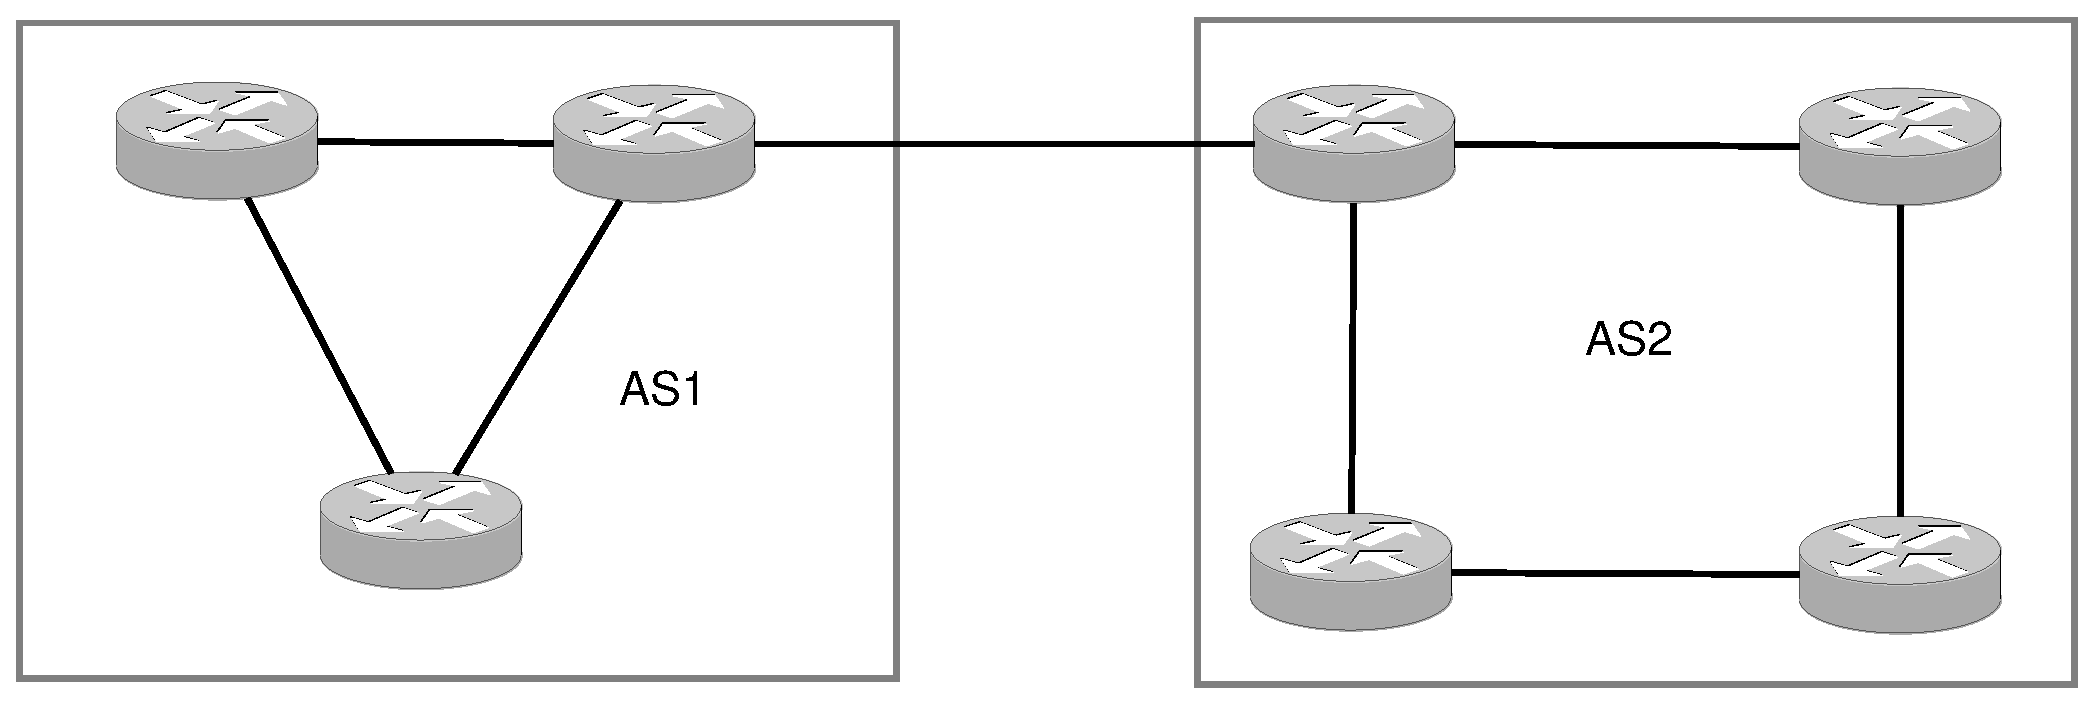
\includegraphics[width=0.8\textwidth]{graphics/as_example.eps}
    \caption{Interconnected autonomous systems}
    \label{fig:as_example}
\end{figure}

Autonomous system concept is used to denote such such networks. The routers those networks interact
through are commonly referred to as autonomous system border routers\footnote{OSPF protocol uses
``autonomous system border router'' (ASBR) as a technical term with specific meaning.} (or, interchangeably, edge routers).

Routing policy mentioned above can be defined solely by router configuration or formally specified and stored in 
a public database, such as whois database.

\section{Types of autonomous systems}

Autonomous systems can be \emph{single-homed} or \emph{multi-homed}. Multi-homed AS is an AS that has connections to more than
one other AS. Single-homed AS is sometimes referred to as ``stub AS''.

Autonomous system is a \emph{transit autonomous system} if it allows traffic from other autonomous systems to pass through it.
A single-homed AS obviously can not be a transit AS. Multi-homed autonomous systems can be but do not have to be transit.
Every AS is free to decide which other autonomous systems it allows traffic from. Technically it is achieved by advertising
or not advertising routes learnt from other autonomous systems.

\begin{figure}[t]
    \centering
    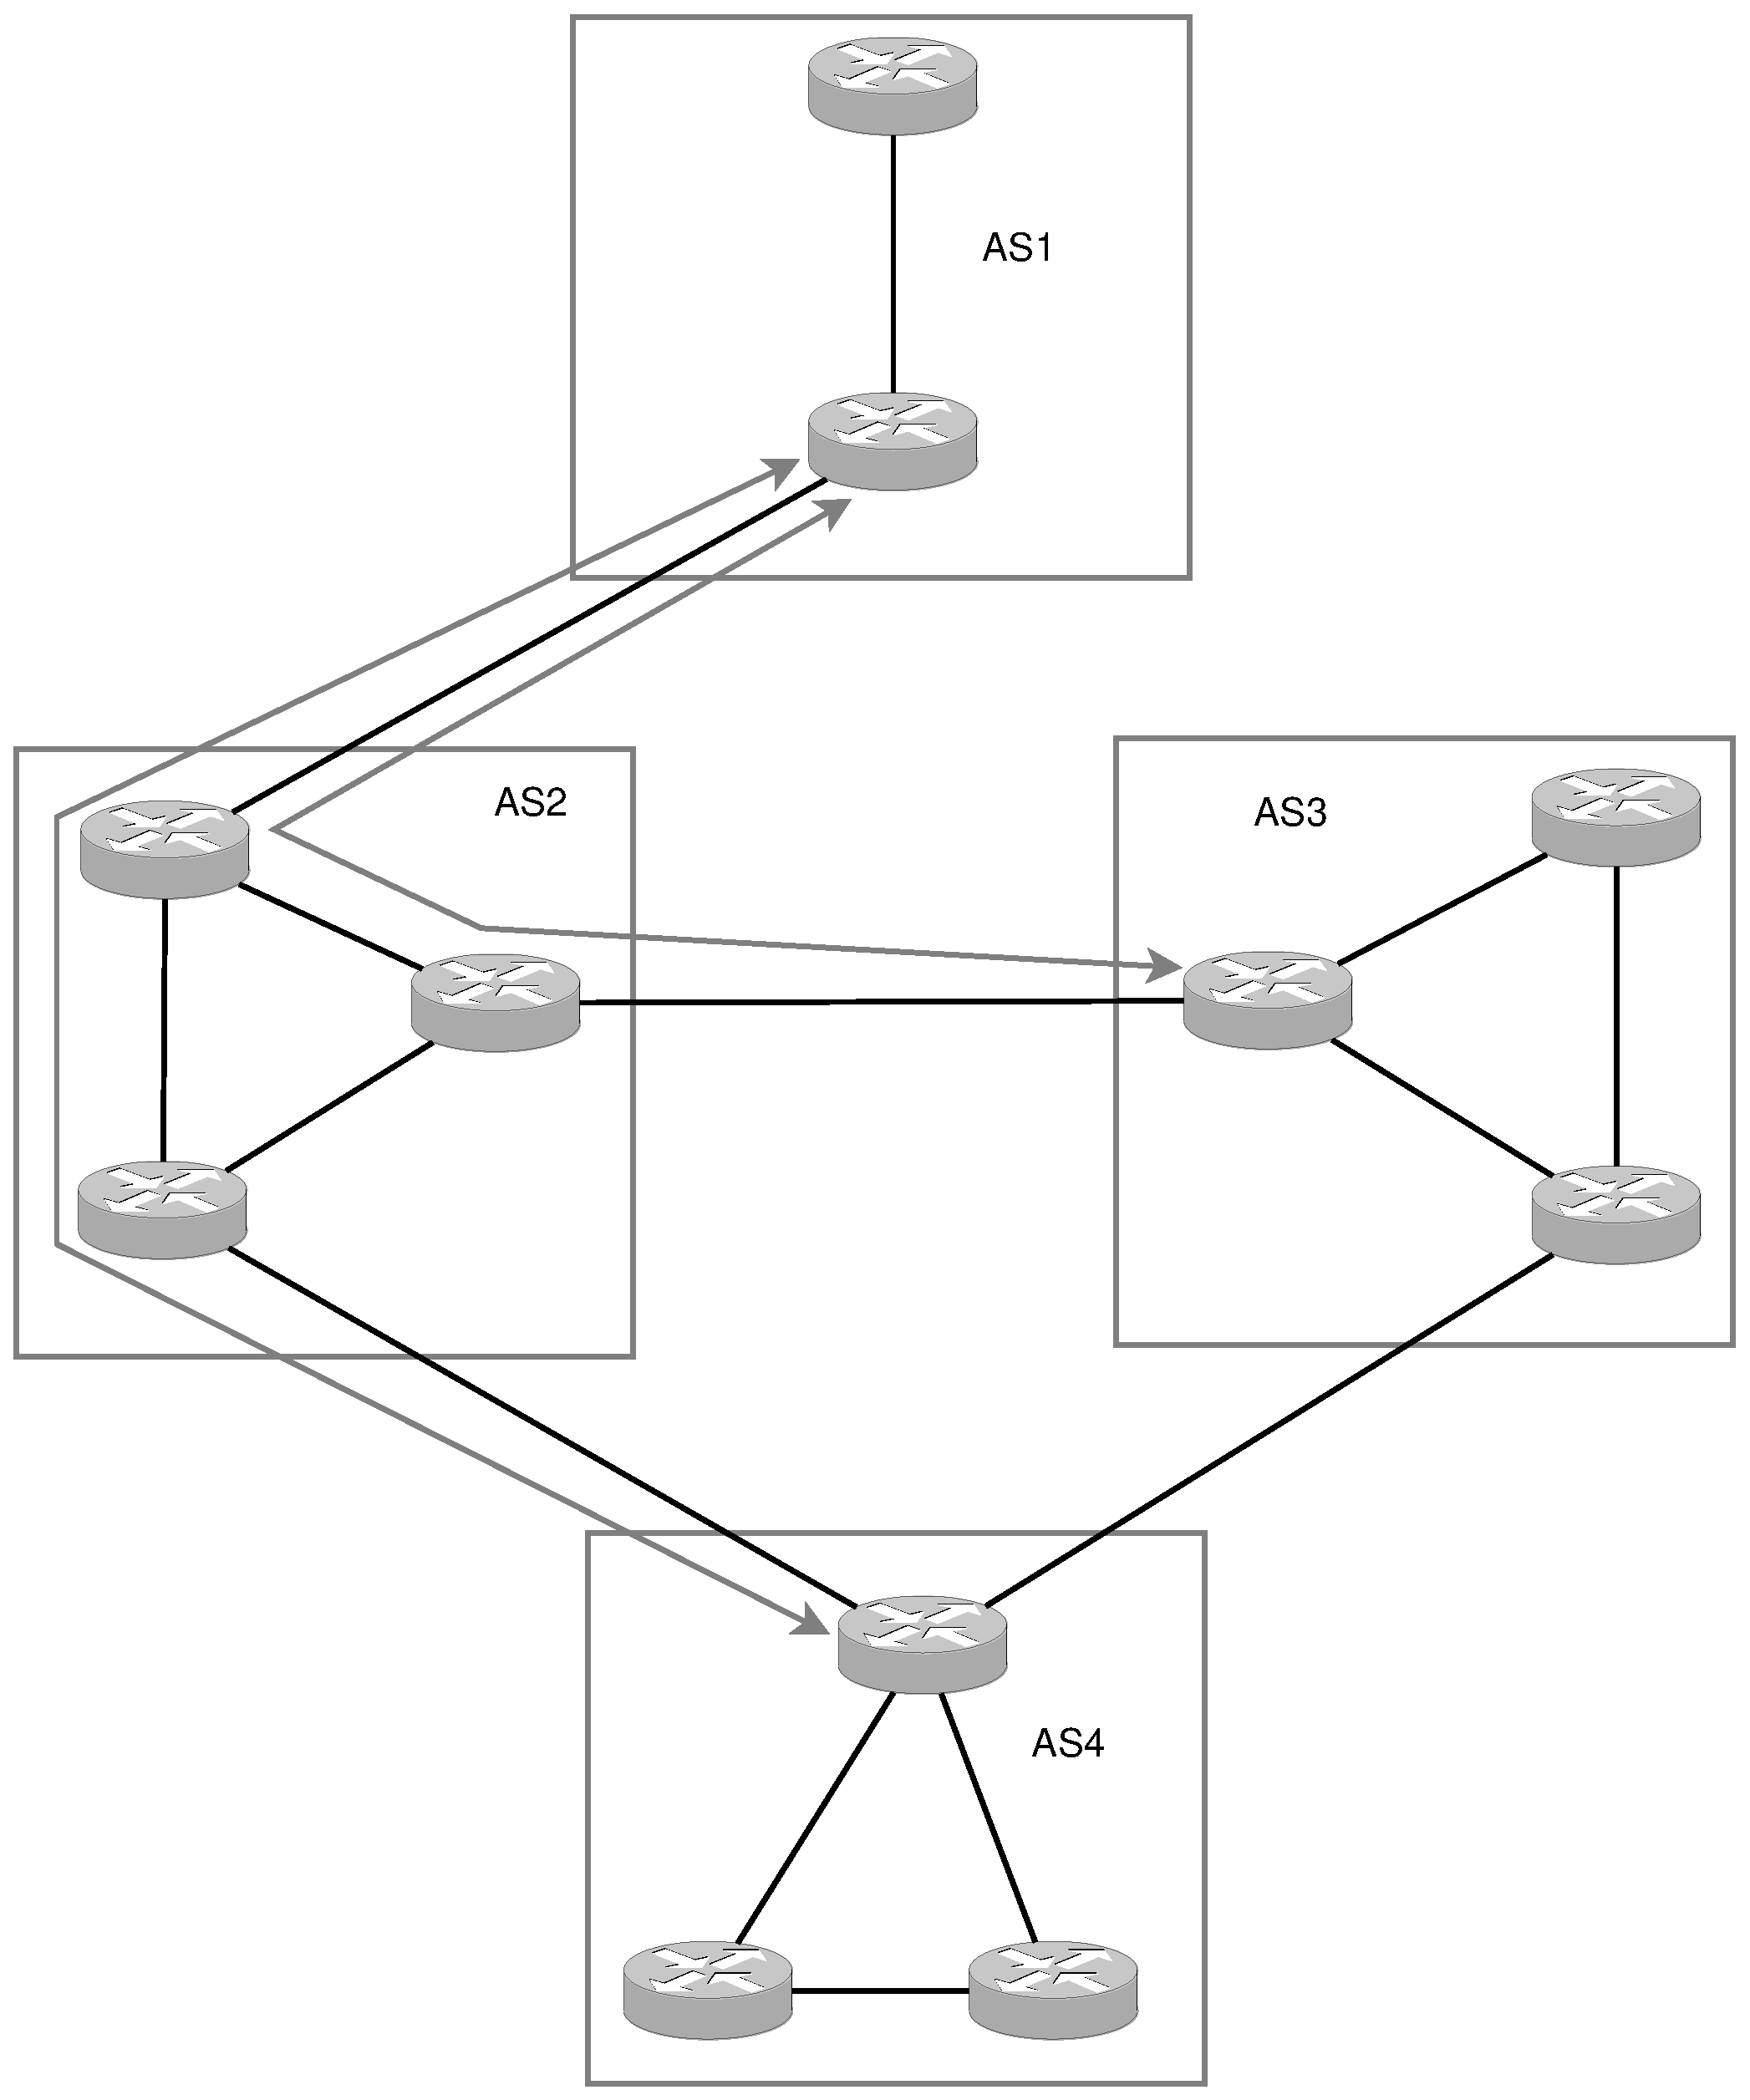
\includegraphics[width=0.8\textwidth]{graphics/as_types.eps}
    \caption{Autonomous systems of different types}
    \label{fig:as_types}
\end{figure}

At the figure above AS1 is a stub AS, because it is connected to only one another AS, AS2. AS2 is both multi-homed
and transit because it is connected to all other autonomous systems and allows traffic from AS1 and AS3 to flow through it,
as gray arros suggest. AS3 and AS4 are multi-homed, but not transit. Note that AS2 is not a transit AS for AS4 relative to
AS3---autonomous systems do not have to treat all other autonomous systems equally.

\section{AS numbers}

From technical point of view, an \emph{autonomous system} (AS) is a group of BGP routers that use the same
\emph{autonomous system number} (ASN). ASN is a required configuration parameter in every BGP implementation.

Autonomous system number is an unsigned 32-bit number, so it can take values from 1 to 4294967294.
Before 2007 16-bit numbers were used but rapid growth of the Internet required range expansion\cite{rfc6793}.
Older BGP implementations may not have 32-bit AS number support, but backwards compatibility mechanisms allow
them to receive routing information from implementations that use 32-bit AS numbers, with some limitations.

Organizational side is more complex. ASN must be unique within its visibility scope to ensure proper
operation of the routing protocol, so there must be a way to ensure uniqueness.

In private internets that do not directly communicate routing information to the Internet the administrator is
responsible for ASN distribution. Technically it is not impossible to use any numbers such as 123,
but it is recommended to use numbers from a special ranges reserved for private use, 64512 to 65535 for
16-bit\cite{rfc1930} and 4200000000 to 4294967294 for 32-bit\cite{rfc6996}.

Two other ranges of AS numbers are reserved for examples and documentation, 64496 to 64511 for 16-bit and
65536 to 65551 for 32-bit\cite{rfc5398}.

Private autonomous systems that use BGP for internal routing do not have to be completely isolated from the Internet,
they only must not include AS numbers from private ranges in routing information sent to Internet peers. Using private
numbers inside the network and globally unique numbers on border routers that advertise network as a whole to the Internet
is a common practice.

Globally unique AS numbers for use in the Internet are assigned by IANA and Regional Internet Registries (RIRs): AfriNIC, APNIC,
ARIN, LACNIC, and RIPE NCC. Registration procedure details depend on the RIR, but generally it requires explanation why
an AS is needed and a yearly registration fee. Typically a company will request an IP address block at the same time.
In case of those autonomous systems registered by RIRs, the routing policy is formally defined and stored in WHOIS database.

\section{Choosing between public and private AS}

Whether you need to apply for a public ASN registration depends on your network setup and use cases.

For multihomed autonomous systems a public ASN is the only option. Single-homed autonomous systems may or may not
have a public ASN.

If you are planning to use redundant connections to the same IP operator, some operators may require a public ASN,
other may use a private ASN for interfacing with your network and advertise your network address on your behalf.

If you are planning to use BGP internally, e.g. inside a VPN, there is no need for public ASN.
